\newpage
\lecture{9}{Лекция 9}
\section{Классификация состояний однородных дискретных марковских цепей}
\begin{Des}
    \begin{align*}
      & p_{ij} = \PP \left( X_n = j \mid X_0 = i \right), \ n \geq 0
    \end{align*}
    $i, j \in S$, $S$~--- конечное или счетное~--- множество состояний.
\end{Des}
\begin{Def}
    Если
    \begin{align*}
      & \exists n \in \NN: \ p_{ij}(n) > 0
    \end{align*}
    то говорят, что \textbf{за $i$ следует $j$} (пишут $i \rightarrow j$).
\end{Def}
Отношение следования \textit{нерефлексивно, несимметрично, транзитивно}.
\begin{Def}
    Если $i \rightarrow j$ и $j \rightarrow i$, то говорят, что \textbf{$i$ и
      $j$~--- сообщающиеся} (пишут $i \leftrightarrow j$).
\end{Def}
Формальнее:
\begin{align*}
  & i \leftrightarrow j \Leftrightarrow \left( \exists n \in \NN: \ p_{ij}(n) > 0\right) \wedge \left( \exists m \in \NN: \ p_{ji}(m) > 0\right)
\end{align*}
Отношение следования \textit{нерефлексивно, симметрично, транзитивно}. Отношение
делит цепь на \textbf{классы сообщающихся состояний} (но это не классы
эквивалентности!).
\begin{Def}
    Если
    \begin{align*}
      \forall j \in S \ (i \rightarrow j) \rightarrow (j \rightarrow i)
    \end{align*}
    то говорят, что \textbf{$i$~--- существенное состояние}, иначе
    \textbf{несущественное}.
\end{Def}
\begin{theorem}
    ~
    \\
    За существенным состоянием может следовать только существенное состояние.
\end{theorem}
\begin{proof}
    ~
    \\
    Пусть $i$~--- существенное, $i \rightarrow j$. Если есть состояние $k$, для
    которого $j \rightarrow k$, то $i \rightarrow k$ в силу транзитивности
    следования, но тогда снова в силу транзитивности будет и $k \rightarrow j$
    (через $i$).
    \\
    ч.~т.~д.
\end{proof}
Цепь делится на \textbf{классы существенных} и \textbf{множество несущественных}
состояний: $S_0$ и $S_1$, $S_2$, $\dots$ (может быть конечное или счетное
число).
\begin{example}~
    \\
    \FloatBarrier
    \begin{center}
        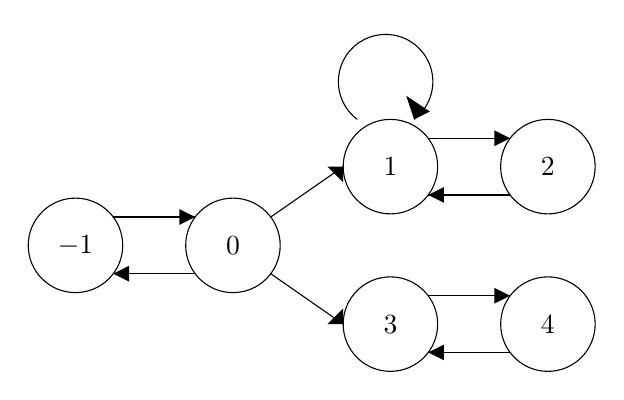
\begin{tikzpicture}[scale=0.2]
            \tikzstyle{every node}+=[inner sep=0pt]
            \draw [black] (0.0, 0.0) circle (3.0);
            \draw [black] (10.0, 0.0) circle (3.0);
            \draw [black] (20.0, 5.0) circle (3.0);
            \draw [black] (30.0, 5.0) circle (3.0);
            \draw [black] (20.0, -5.0) circle (3.0);
            \draw [black] (30.0, -5.0) circle (3.0);
            \draw [black] (2.4, 1.8) -- (7.6, 1.8);
            \draw [black] (7.6, -1.8) -- (2.4, -1.8);
            \draw [black] (12.4, 1.8) -- (17, 5);
            \draw [black] (12.4, -1.8) -- (17, -5);
            \draw [black] (22.4, 6.8) -- (27.6, 6.8);
            \draw [black] (22.4, -6.8) -- (27.6, -6.8);
            \draw [black] (27.6, 3.2) -- (22.4, 3.2);
            \draw [black] (27.6, -3.2) -- (22.4, -3.2);
            \draw [black] (21.5, 8.0) arc (-53.0:233.0:3.0);
            \draw (0.0, 0.0) node {$-1$};
            \draw (10.0, 0.0) node {$0$};
            \draw (20.0, 5.0) node {$1$};
            \draw (30.0, 5.0) node {$2$};
            \draw (20.0, -5.0) node {$3$};
            \draw (30.0, -5.0) node {$4$};
            \fill [black] (7.6, 1.8) -- (6.6, 2.3) --(6.6, 1.3);
            \fill [black] (2.4, -1.8) -- (3.4, -2.3) --(3.4, -1.3);
            \fill [black] (27.6, 6.8) -- (26.6, 7.3) --(26.6, 6.3);
            \fill [black] (22.4, -6.8) -- (23.4, -7.3) --(23.4, -6.3);
            \fill [black] (27.6, -3.2) -- (26.6, -2.7) --(26.6, -3.7);
            \fill [black] (22.4, 3.2) -- (23.4, 2.7) --(23.4, 3.7);
            \fill [black] (21.5, 8.0) -- (22.5, 8.5) --(21.0, 9.5);
            \fill [black] (17.0, 5.0) -- (16.0, 5.0) --(17.0, 4.0);
            \fill [black] (17.0, -5.0) -- (16.0, -5.0) --(17.0, -4.0);
        \end{tikzpicture}
    \end{center}
    \FloatBarrier
    В данной цепи $S_0 = \{-1, 0\}$, $S_1 = \{1,2\}$, $S_2 = \{3,4\}$. (Любые
    вероятности над стрелками так, чтобы сумма исходящих была единицей для каждой
    вершины, подойдут для конкретизации).
\end{example}
\begin{Def}
    Если все состояния сообщаются, то цепь называется \textbf{неразложимой
      (неприводимой)}.
\end{Def}
\begin{Prop}
    ~
    \\
    Всякая марковская цепь может быть представлена в виде совокупности
    неприводимых цепей и множества несущественных состояний.
    \\
    По их поведению однозначно восстанавливается поведение цепи.
\end{Prop}
\begin{Des}
    Вероятность первого попадания из $i$ в $i$ за $n$ шагов обозначается как
    \begin{align*}
      & f_i (n) = \PP \left\{ X_n = 1, \forall m \in \{1, \dots, n-1\} \ X_m \neq i \mid X_0 = i\right\} = \PP \left\{ X_n = 1, X_{<n} \neq i \mid X_0 = i\right\}, \ n \geq 1
    \end{align*}
\end{Des}
\begin{Note}
    \begin{align*}
      & f_i(n) \leq p_{ii}(n) = \PP(X_n = i \mid X_0 = i)
    \end{align*}
    но далеко не факт, что выполняется равенство.
\end{Note}
\begin{Note}
    \begin{align*}
      & p_{ii}(n) = \sum_{m=1}^nf_i(m)p_{ii}(n-m)
    \end{align*}
\end{Note}
\begin{proof}
    ~
    \\
    Пусть
    \begin{align*}
      & A_m = \left\{ X_m = i, X_{<m} \neq i \right\}
    \end{align*}
    Тогда
    \begin{align*}
      & p_{ii}(n) = \PP(X_n = i \mid X_0 = i) = \sum_{m=1}^n \PP(A_m, X_n = i \mid X_0 = i) = \sum_{m=1}^n \left( X_m=i, X_{<m} \neq i, X_n = i \mid \right. \\
      & \left. \mid X_0 = i \right) = \sum_{m=1}^n \PP(X_n = i \mid X_0 = i, X_m = i, X_{<m} \neq i)\PP(X_m = i, X_{<m} \neq i \mid X_0 = i) = \text{\textit{в силу}} \\
      & \text{\textit{марковости}} = \sum_{m=1}^n \PP(X_n = i \mid X_m = i) \PP (X_m = i, X_{<m} = i \mid X_0 = i) = \sum_{m=1}^n p_{ii}(n-m) f_i(m)
    \end{align*}  
\end{proof}
\begin{Des}
    Обозначим вероятность возврата в $i$ за конечное число шагов
    \begin{align*}
      & F_i = \sum_{n=1}^{\infty}f_i (n)
    \end{align*}
\end{Des}
\begin{Def}
    Если $F_i = 1$, то состояние $i$ наывается \textbf{возвратным}, иначе
    \textbf{невозвратным}.
\end{Def}
\begin{theorem}
    ~
    \\
    $i$~--- возвратное состояние тогда и только тогда, когда
    \begin{align*}
      & R_i = \sum_{m=1}^\infty p_{ii}(n) = \infty
    \end{align*}
\end{theorem}
\begin{proof}
    ~
    \\
    Известно, что
    \begin{align*}
      & p_{ii}(n) = \sum_{m=1}^n p_{ii}(n-m) f_i(m)
    \end{align*}
    Переобозначая:
    \begin{align*}
      & p_{ii}(n) = v_n, \ u_m = f_i(m), \ v_0 = 1, \ u_0 = 0
    \end{align*}
    получаем
    \begin{align*}
      & v_n = \sum_{m=0}^n u_mv_{n-m}
    \end{align*}
    Введем функции:
    \begin{align*}
      & V(z) = \sum_{k=0}^\infty v_kz^k, \ U(z) = \sum_{k=0}^\infty u_kz^k
    \end{align*}
    Отсюда
    \begin{align*}
      & V(z) - 1 = U(z)V(z)
    \end{align*}
    \begin{align*}
      & V(z) = \frac{1}{1-U(z)}, \ U(z) = \frac{V(z) - 1}{V(z)}
    \end{align*}
    Из математического анализа известна теорема Абеля:
    \\
    \textit{ряд из неотрицательных $a_k$ сходится к конечному $a$ тогда и только
      тогда, когда существует предел}
    \begin{align*}
      & \lim_{z \to 1-0}\sum_{k=0}^\infty a_k z^k = a
    \end{align*}
    Используем эту теорему и получим, что:
    \begin{align*}
      & U(1) = \sum_{k=1}^\infty u_k = F_i = 1 \Rightarrow \lim_{z \to 1-0} V(z) = \infty \Rightarrow R_i = \sum_{n=1}^\infty p_{ii}(n) = \infty
    \end{align*}
    \begin{align*}
      & R_i = \sum_{n=1}^\infty p_{ii}(n) = \infty \Rightarrow \lim_{z \to 1-0} V(z) = \infty \Rightarrow U(1) = \sum_{k=1}^\infty u_k = F_i = 1 
    \end{align*}
    ч.~т.~д.
\end{proof}
\begin{Def}
    Если $\dst \lim_{n \to \infty} p_{ii}(n) = 0$, то состояние $i$ называется
    \textbf{нулевым}, иначе \textbf{ненулевым}.
\end{Def}
\begin{Prop}
    ~
    \\
    Если состояние невозвратное, то оно нулевое. Если состояние ненулевое, то
    оно возвратное.
\end{Prop}
\begin{proof}
    ~
    \\
    Второе утверждение означает, что $n$-й член ряда из критерия возвратности не
    стремится к нулю. Значит, ряд, очевидно, расходится, и состояние
    невозвратно.
    \\
    Первое утверждение равносильно второму (контрапозиция).
\end{proof}
\begin{Def}
    Если $i \rightarrow i$, то НОД множества положительных $n$ таких, что
    $p_{ii}(n) > 0$, называется \textbf{периодом состояния $i$} (пишут $d_i$).
\end{Def}
\begin{Def}
    Если $d_i > 1$, то состояние $i$ называется \textbf{периодическим с периодом
    $d_i$}; если $d_i=1$~--- \textbf{непериодическим} (редко
  \textbf{периодическим с периодом $1$}).
\end{Def}
\begin{example}~
    \\
    \FloatBarrier
    \begin{center}
        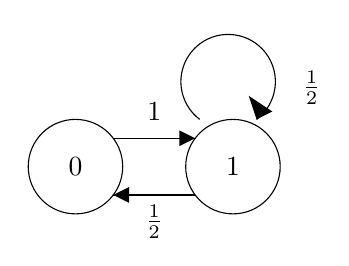
\begin{tikzpicture}[scale=0.2]
            \tikzstyle{every node}+=[inner sep=0pt]
            \draw [black] (10.0, 5.0) circle (3.0);
            \draw [black] (20.0, 5.0) circle (3.0);
            \draw [black] (12.4, 6.8) -- (17.6, 6.8);
            \draw [black] (17.6, 3.2) -- (12.4, 3.2);
            \draw [black] (21.5, 8.0) arc (-53.0:233.0:3.0);
            \draw (10.0, 5.0) node {$0$};
            \draw (20.0, 5.0) node {$1$};
            \fill [black] (17.6, 6.8) -- (16.6, 7.3) --(16.6, 6.3);
            \fill [black] (12.4, 3.2) -- (13.4, 2.7) --(13.4, 3.7);
            \fill [black] (21.5, 8.0) -- (22.5, 8.5) --(21.0, 9.5);
            \draw (15.0, 8.5) node {$1$};
            \draw (15.0, 1.5) node {$\frac{1}{2}$};
            \draw (25.0, 10.0) node {$\frac{1}{2}$};
        \end{tikzpicture}
    \end{center}
    \FloatBarrier
    В данной цепи оба состояние непериодические: $p_{11}(1) = \dst \frac{1}{2}
    \neq 0$, поэтому это верно для $1$; $p_{00}(2) = \dst \frac{1}{2} \neq 0$,
    $p_{00}(3) = \dst \frac{1}{4} \neq 0$, $\GCD(2,3) = 1$, поэтому это верно
    для $0$.
\end{example}
\begin{theorem} (о солидарности)
    \\
    Для неразложимых марковских цепей выполняется:
    \begin{enumerate}
        \item Если есть хотя бы одно нулевое состояние, то нулевыми будут все;
        \item Если есть хотя бы одно возвратное состояние, то возвратными будут
        все;
        \item Если есть хотя бы одно состояние с периодом $d \geq 1$, то такой
        же период будут иметь все.
    \end{enumerate}
\end{theorem}
\begin{proof}
    ~
    \\
    Рассмотрим произвольные $i$, $j$. В силу неразложимости они сообщаются;
    соответственно,
    \begin{align*}
      & \exists M > 0, \ \exists N > 0: \ \alpha = p_{ij}(M) > 0, \ \beta = p_{ji}(N) > 0
    \end{align*}
    \begin{enumerate}
        \item Можем записать:
        \begin{align*}
          & p_{ii}(M+n+N) = \sum_{k \in S}\sum_{l \in S} p_{ik}(M)p_{kl}(n)p_{li}(N) \geq p_{ij}(M)p_{jj}(N) = \alpha \beta p_{jj}(n)
        \end{align*}
        Аналогично
        \begin{align*}
          & p_{jj}(M+n+N) = \alpha \beta p_{ii}(n)
        \end{align*}
        Итак, стремление к нулю $p_{ii}(n)$ и $p_{jj}(n)$ равносильно в силу
        фиксированности $\alpha$, $\beta$ (что по определению означает, что $i$
        и $j$ нулевые либо ненулевые вместе).
        \item Пусть $j$ для определенности возвратно. Тогда по критерию
        возвратности
        \begin{align*}
          & \sum_{n=1}^\infty p_{jj}(n) = \infty
        \end{align*}
        Можем записать:
        \begin{align*}
          & \sum_{n=1}^\infty p_{ii}(M+n+N) \geq \alpha \beta \sum_{n=1}^\infty p_{jj}(n) \infty
        \end{align*}
        Соответственно, $i$ является возвратным.
        \item Пусть
        \begin{align*}
          & W_i = \{n \mid p_{ii}(n) > 0\}, \ d_i = \GCD(W_i), \ W_j = \{m \mid p_{jj}(m) > 0\}, \ d_j = \GCD(W_j)
        \end{align*}
        Заметим: $M+N \in W_i \cap W_j$. Рассмотрим теперь $W = \{M+N+n\}$, $n
        \in W_i$. Тогда
        \begin{align*}
          & p_{jj}(M+n+N) \geq \alpha \beta p_{ii}(n) > 0 \Rightarrow M+N+n \, \vdots \, d_i \Rightarrow M+N+n \in W_j \Rightarrow \\
          & M+N+n \, \vdots \, d_j \Rightarrow d_j \leq d_i
        \end{align*}
        Аналогично можно показать, что $d_i \leq d_j$. Итак, периоды равны.
    \end{enumerate}
\end{proof}
\begin{theorem} (без доказательства)
    \\
    В любой дискретной марковской цепи из несущественности состояния следует его
    невозвратность и, соответственно, из возвратности~--- существенность.
\end{theorem}
\begin{theorem} (без доказательства)
    \\
    В любой конечной дискретной неразложимой марковской цепи все состояния
    ненулевые и, следовательно, возвратные.
\end{theorem}
\begin{Prop} (без доказательства)
    \\
    В любой конечной дискретной марковской цепи возвратность состояния
    равносильна его существенности, а несущественность невозвратности; из
    невозвратности следует, что состояние нулевое.
\end{Prop}